\section{Evaluation}\label{evaluation}
This section reveals the evaluation of SCache with comprehensive workloads and benchmarks. 
First we run a simple DAG job with single shuffle to analyze hardware utilization and impact of shuffle optimization from the scope of a task to a job. 
Then we use a recognized shuffle intensive benchmark --- Terasort \cite{spark-tera} to evaluate SCache with different data partition schemes.

\begin{figure}
	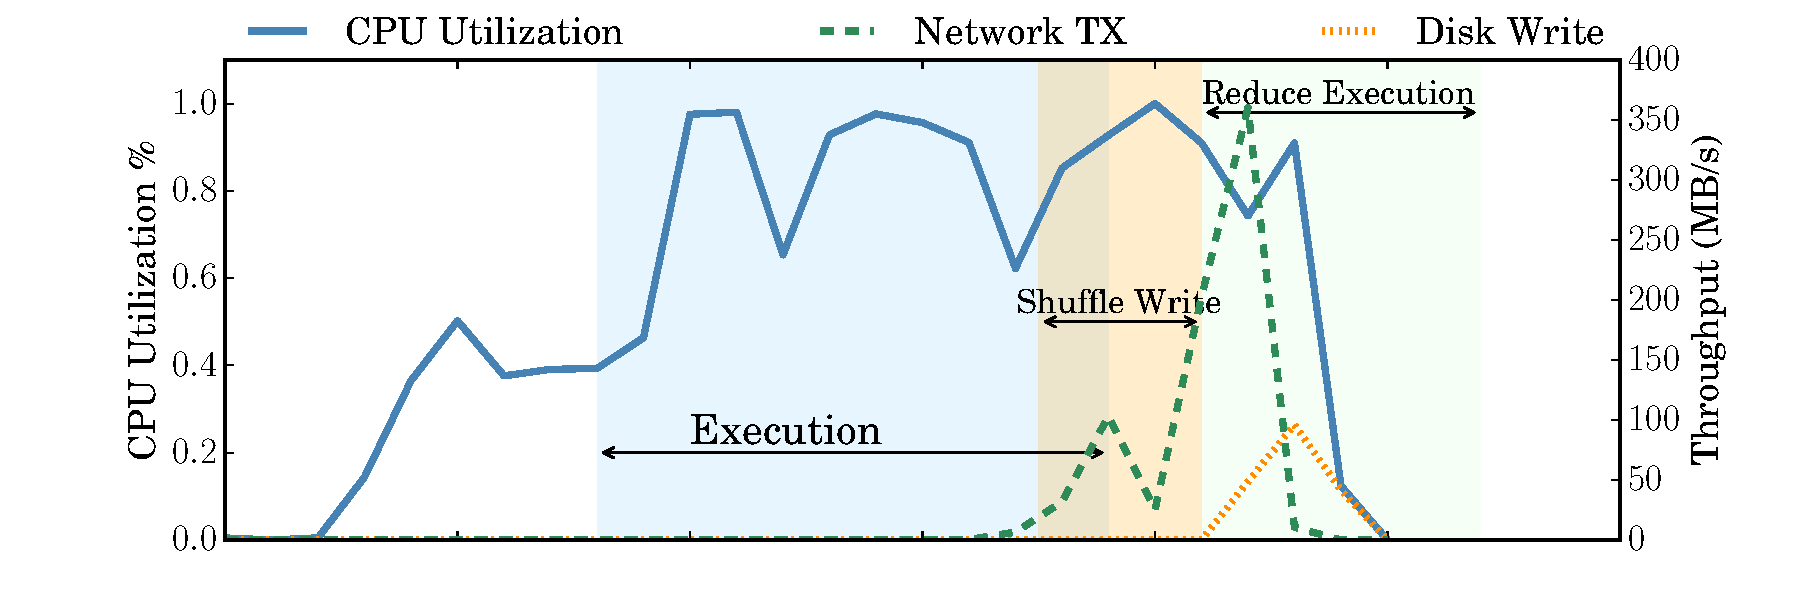
\includegraphics[width=\linewidth]{fig/scache_util}
	\caption{CPU utilization and I/O throughput of a node during a Spark single shuffle application With SCache}
	\label{fig:scache_util}
\end{figure}

In order to prove the performance gain of SCache with a real production workload, we also evaluate Spark TPC-DS \footnote{https://github.com/databricks/spark-sql-perf} and present the overall performance improvement.
{\color{blue}
To prove SCache compatibility as a cross-framework plug-in, we implemented SCache on both Hadoop MapReduce and Spark. 
Due to the simple DAG computing in Hadoop MapReduce, we only use Terasort as a shuffle-heavy benchmark to evaluate the performance of Hadoop Mapreduce with SCache.
}
At last, we measure the overhead of weighted reservoir sampling. 
In short, SCache can decrease ~$89\%$ time of Spark shuffle. Furthermore, SCache achieves a ~$75\%$ and ~$50\%$ improvement of reduce stage completion time respectively in simple DAG application and Terasort without introducing extra network traffic. More impressively, the overall completion time of TPC-DS can be improved ~$40\%$ on average by applying optimization from SCache.
{\color{blue}Meanwhile, Hadoop Mapreduce with Scache optimize job completion time by up to 15\% and an average of 13\%}

% Because a complex Spark application consists of multiple stages. The completion time of each stage varies under different input data, configurations and different number of stages. This uncertainty leads to the dilemma that dramatic fluctuation occurs in overall performance comparison. To present a straightforward illustration, we limit the scope of most evaluations in a single stage.
\begin{figure*}
	\centering
	\begin{minipage}[t]{.32\linewidth}
		\begin{subfigure}{\linewidth}
			\begin{minipage}{\linewidth}
				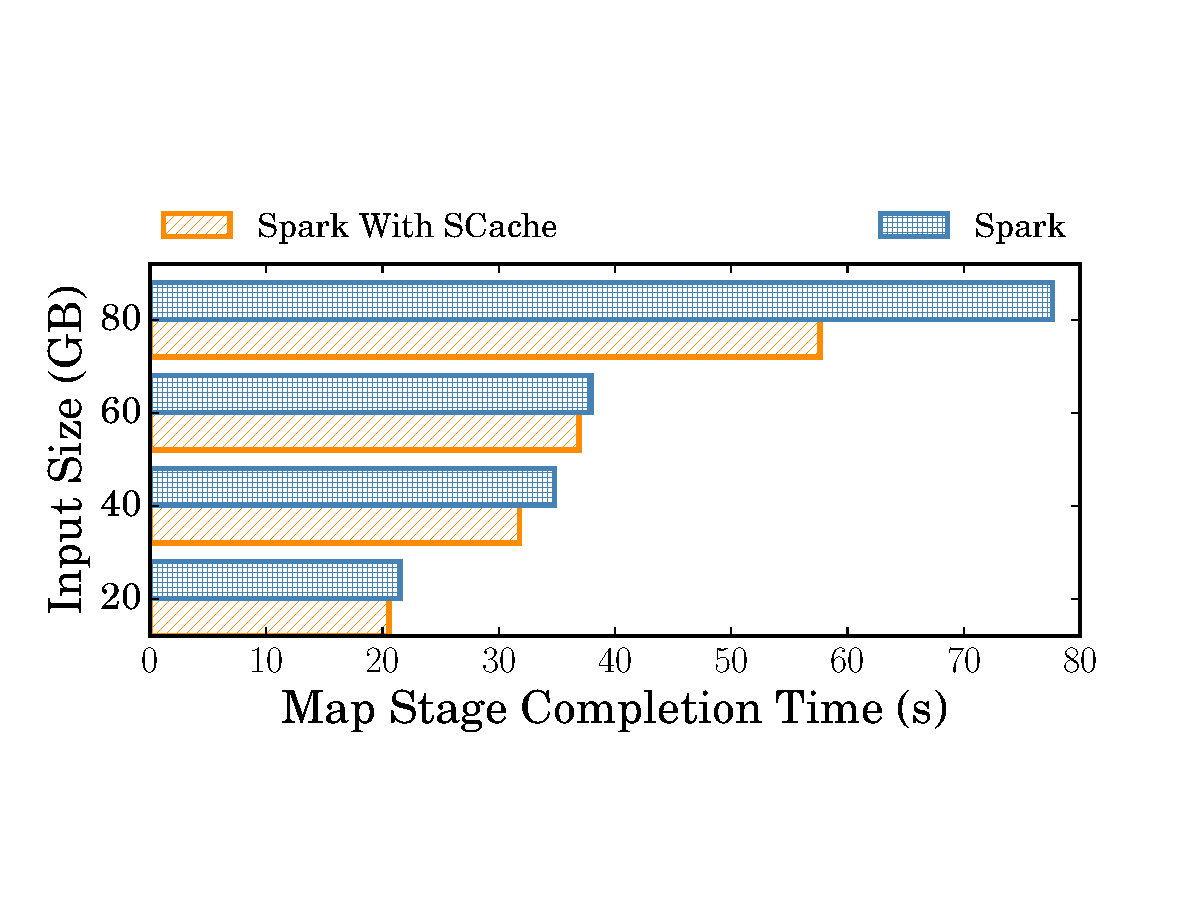
\includegraphics[width=\linewidth]{fig/groupbymapstage}
				\caption{Map Stage Completion Time}
				\label{fig:mapstage}
			\end{minipage}
			\begin{minipage}{\linewidth}
				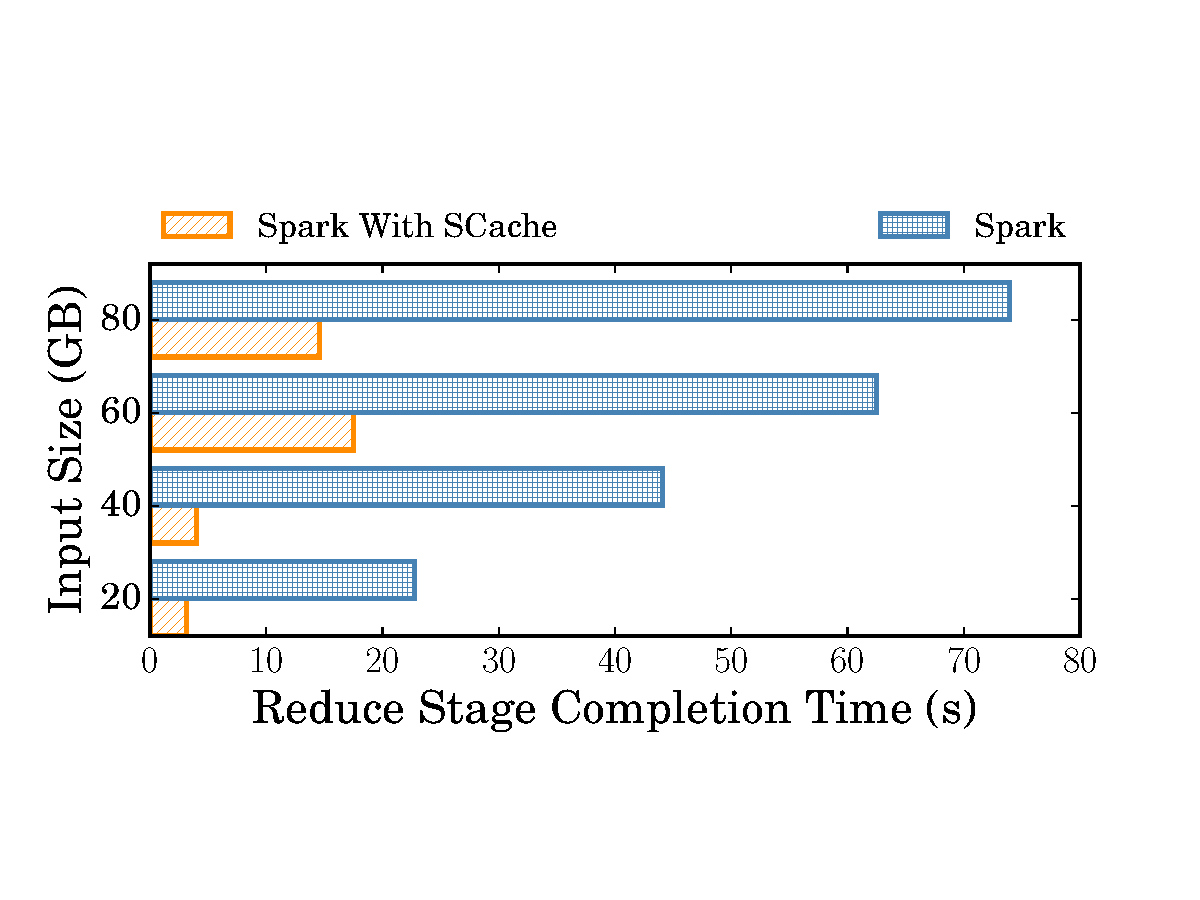
\includegraphics[width=\linewidth]{fig/groupbyreducestage}
				\caption{Reduce Stage Completion Time}
				\label{fig:reducestage}	
			\end{minipage}
		\end{subfigure}
		\caption{Stage Completion Time of Single Shuffle Test}
		\label{fig:singleshuffle}
	\end{minipage}	
	\begin{minipage}[t]{.32\linewidth}
		\begin{subfigure}{\linewidth}
			\begin{minipage}{\linewidth}
				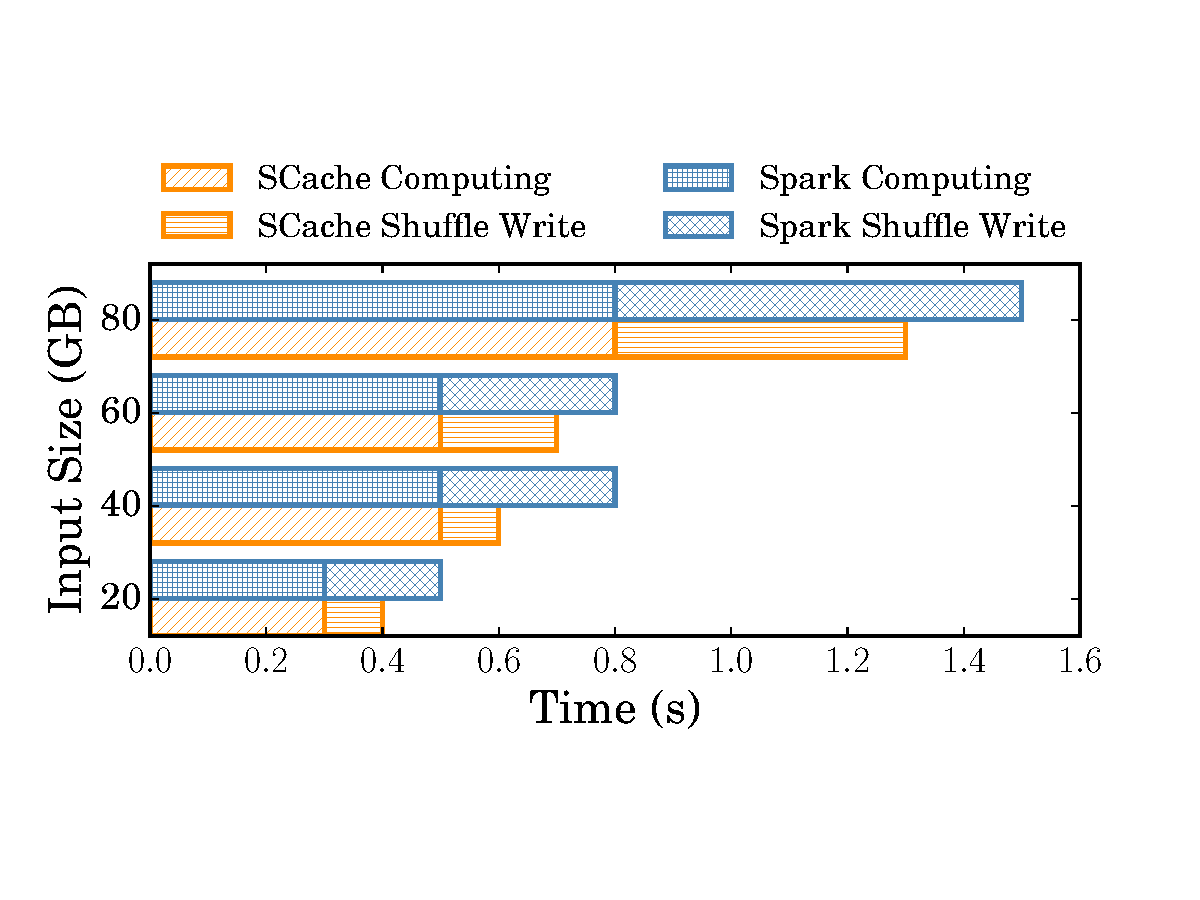
\includegraphics[width=\linewidth]{fig/groupbymaptask}
				\caption{Median Task in Map Stages}
				\label{fig:maptask}
			\end{minipage}

			\begin{minipage}{\linewidth}
				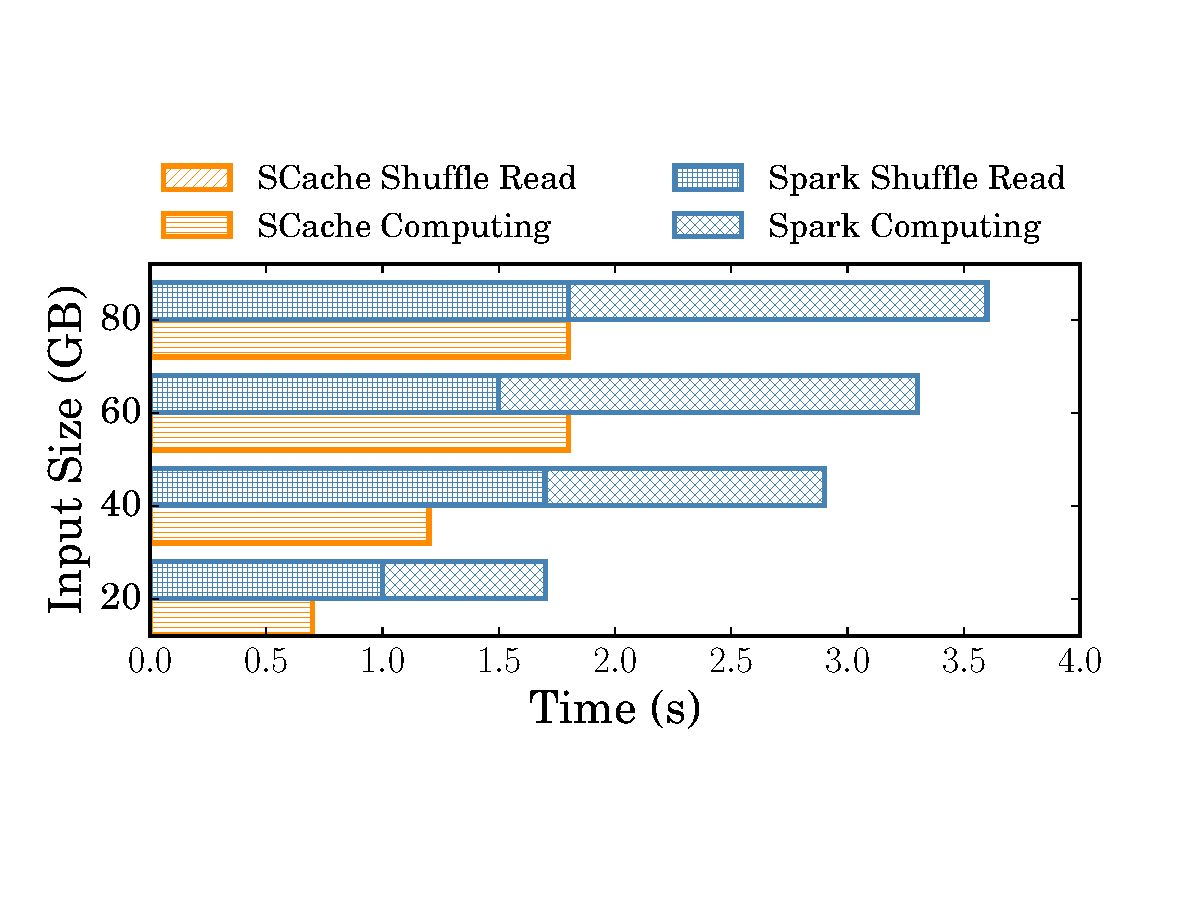
\includegraphics[width=\linewidth]{fig/groupbyreducetask}
				\caption{Median Task in Reduce Stages}
				\label{fig:reducetask}
			\end{minipage}
		\end{subfigure}
		\caption{Median Task Completion Time of Single Shuffle Test}
		\label{fig:singleshuffletask}
	\end{minipage}	
	\begin{minipage}[t]{.32\linewidth}
		\begin{subfigure}{\linewidth}
			\begin{minipage}{\linewidth}
				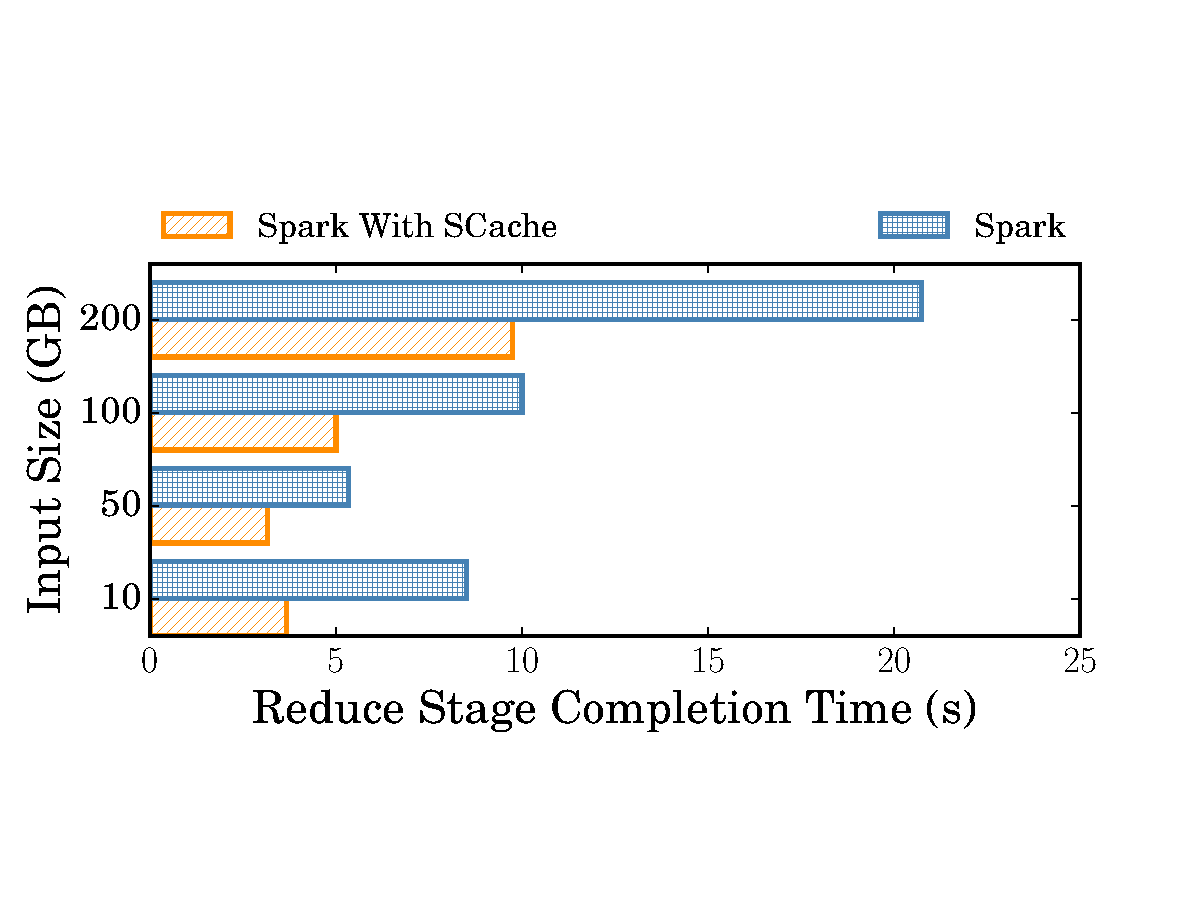
\includegraphics[width=\linewidth]{fig/tera}
				\caption{Reduce Stage of First Shuffle}
				\label{fig:terasort}
			\end{minipage}

			\begin{minipage}{\linewidth}
				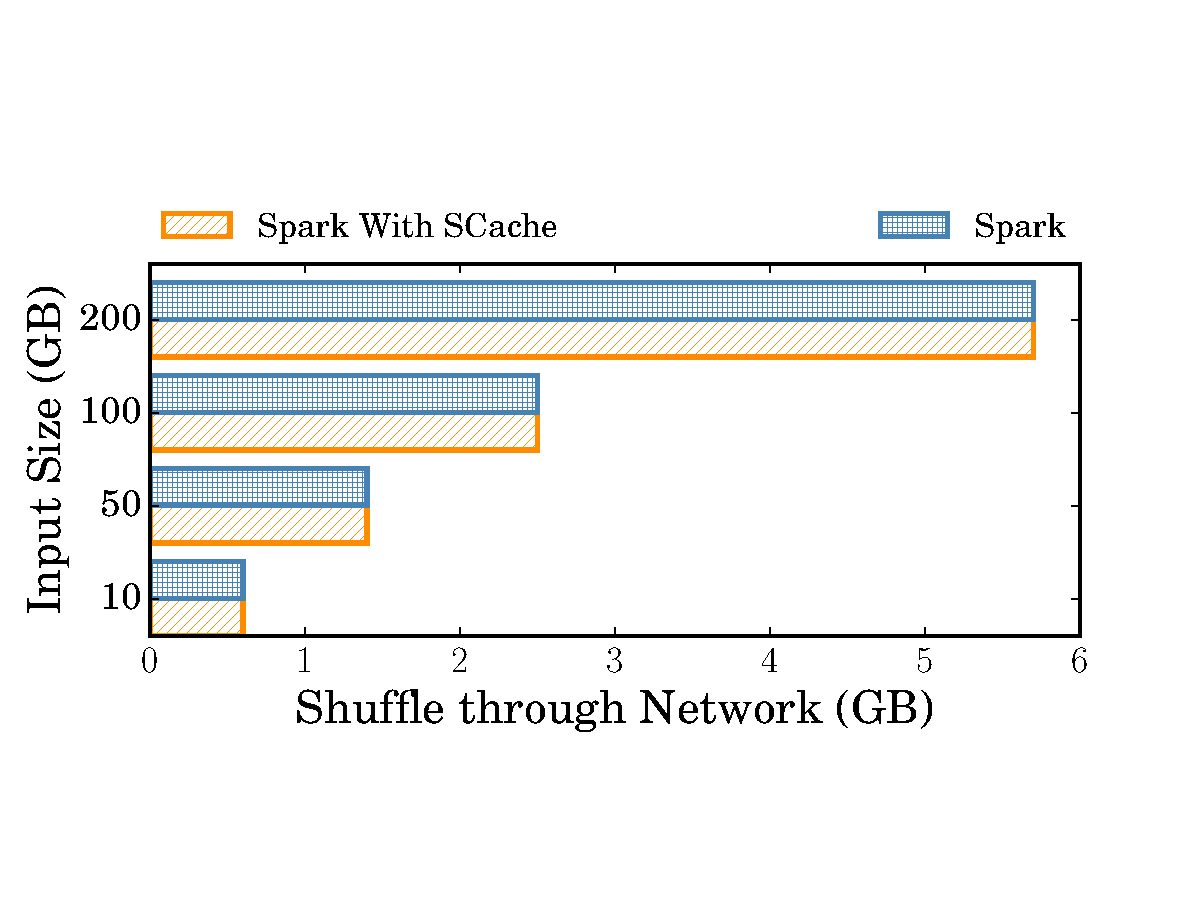
\includegraphics[width=\linewidth]{fig/tera_shuffle}
				\caption{Network Traffic of Second Shuffle}
				\label{fig:terashuffle}
			\end{minipage}
		\end{subfigure}
		\caption{Terasort Evaluation}
	\end{minipage}
\end{figure*}

\subsection{Setup}\label{stepup}
We implement a Spark demon to enable shuffle optimization as a representative.
We run our experiments on a 50 m4.xlarge nodes cluster on Amazon EC2 \footnote{http://aws.amazon.com/ec2/}. Each node has 16GB memory and 4 CPUs. The network bandwidth is not specifically provided by Amazon. Our evaluations reveal the bandwidth is about 300 Mbps (see Figure \ref{fig:util}).

\subsection{Simple DAG Analysis}
%\subsubsection{Hardware Utilization}
We first run the same single shuffle test as mentioned in Figure \ref{fig:util}. As shown in Figure \ref{fig:scache_util}, the hardware utilization is captured from one node during the job. Note that since the completion time of whole job is about $50\%$ less than Spark without SCache, the duration of Figure \ref{fig:scache_util} is cut in half as well. An overlap among CPU, disk, and network can be easily observed in Figure \ref{fig:scache_util}. That is, SCache prevents the computing process from being cutting off by the I/O operations with a fine-grained resource allocation. It ensures the overall CPU utilization of the cluster stays in a high level. In addition, the decoupling of shuffle write helps free the CPU earlier and leads to a faster map task computation. At the same time, the shuffle pre-fetching in the early stage of map phase shifts the network transfer completion time, which decreases reduce stage completion time. The combination is the main performance gain we achieved on the scope of hardware utilization by SCache.
% \begin{figure}
% 	%\vspace*{-0.01cm}
% 	\begin{subfigure}{\linewidth}
% 		\centering
% 		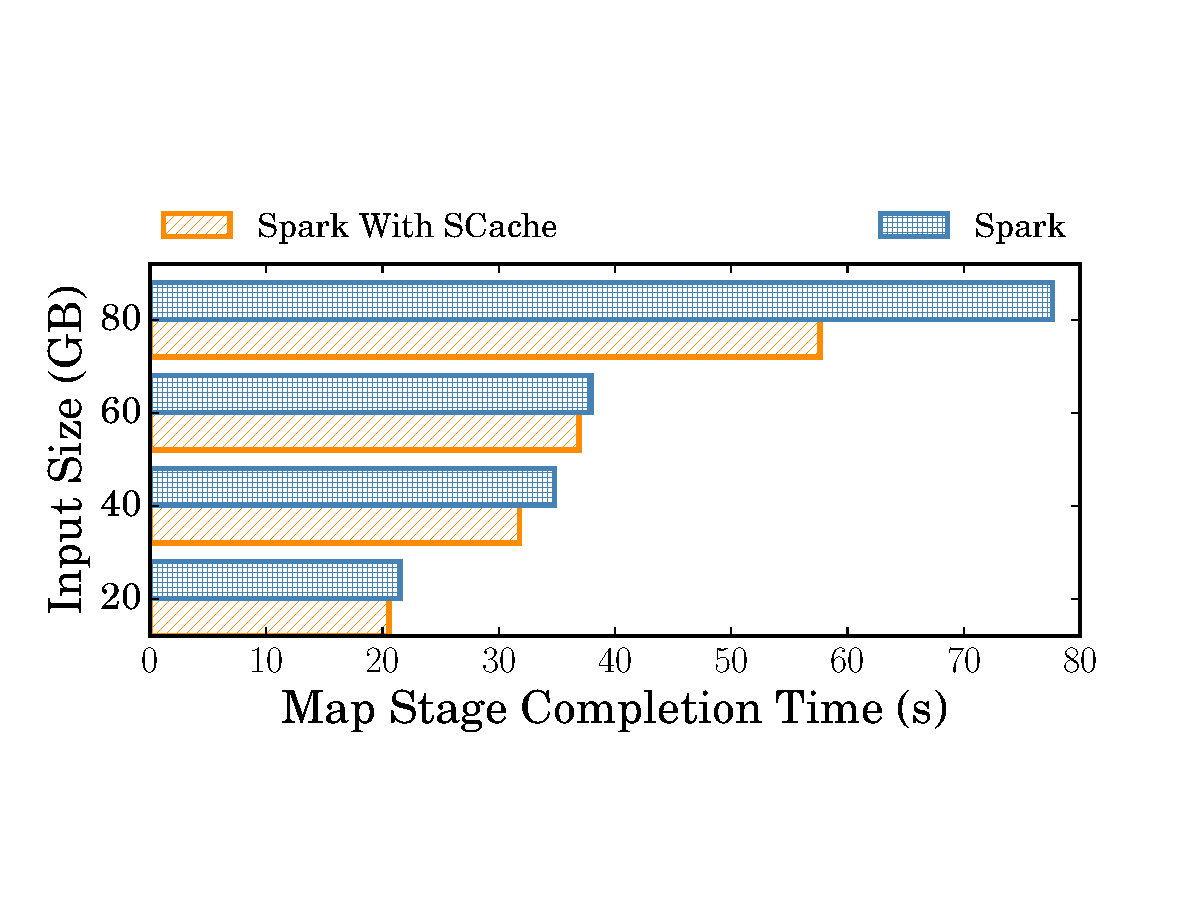
\includegraphics[width=0.6\linewidth]{fig/groupbymapstage}
% 		\caption{Map Stage Completion Time Comparison}
% 		\label{fig:mapstage}
% 	\end{subfigure}
% 	\begin{subfigure}{\linewidth}
% 		\centering
% 		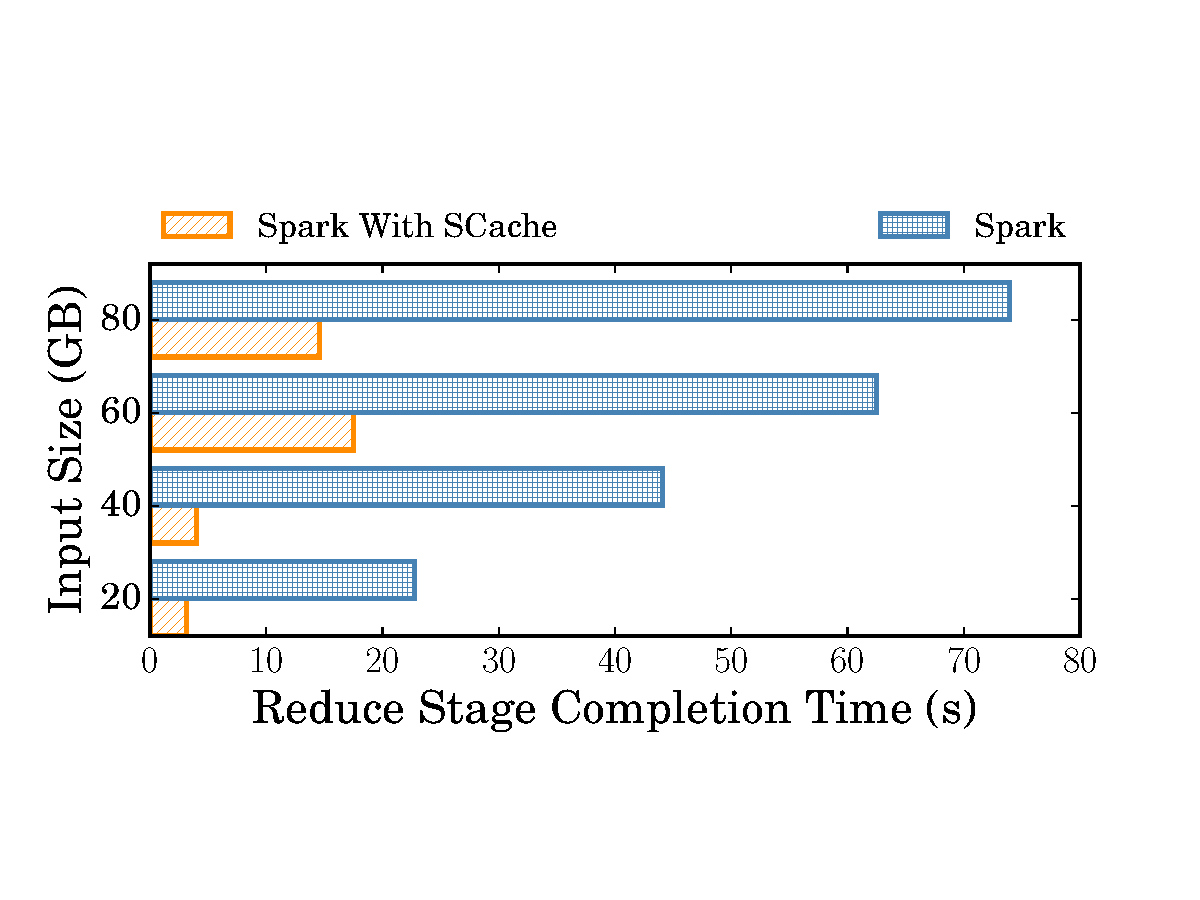
\includegraphics[width=0.6\linewidth]{fig/groupbyreducestage}
% 		\caption{Reduce Stage Completion Time Comparison}
% 		\label{fig:reducestage}
% 	\end{subfigure}
% 	\caption{Stage Completion Time of Single Shuffle Test}
% 	\label{fig:singleshuffle}
% \end{figure}

% \begin{figure}
% 	\begin{subfigure}{\linewidth}
% 		\centering
% 		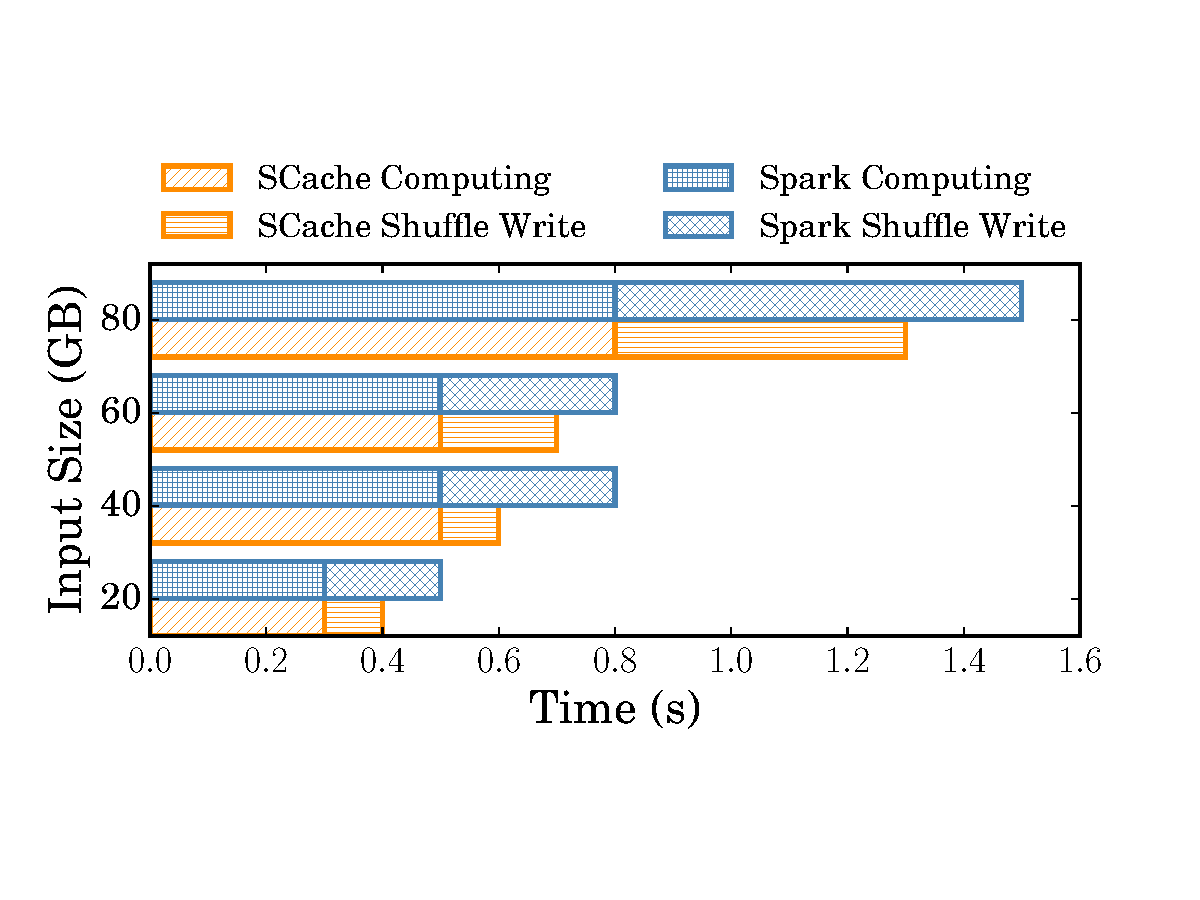
\includegraphics[width=0.6\linewidth]{fig/groupbymaptask}
% 		\caption{Median Task Details in Map Stages}
% 		\label{fig:maptask}
% 	\end{subfigure}
% 	\begin{subfigure}{\linewidth}
% 		\centering
% 		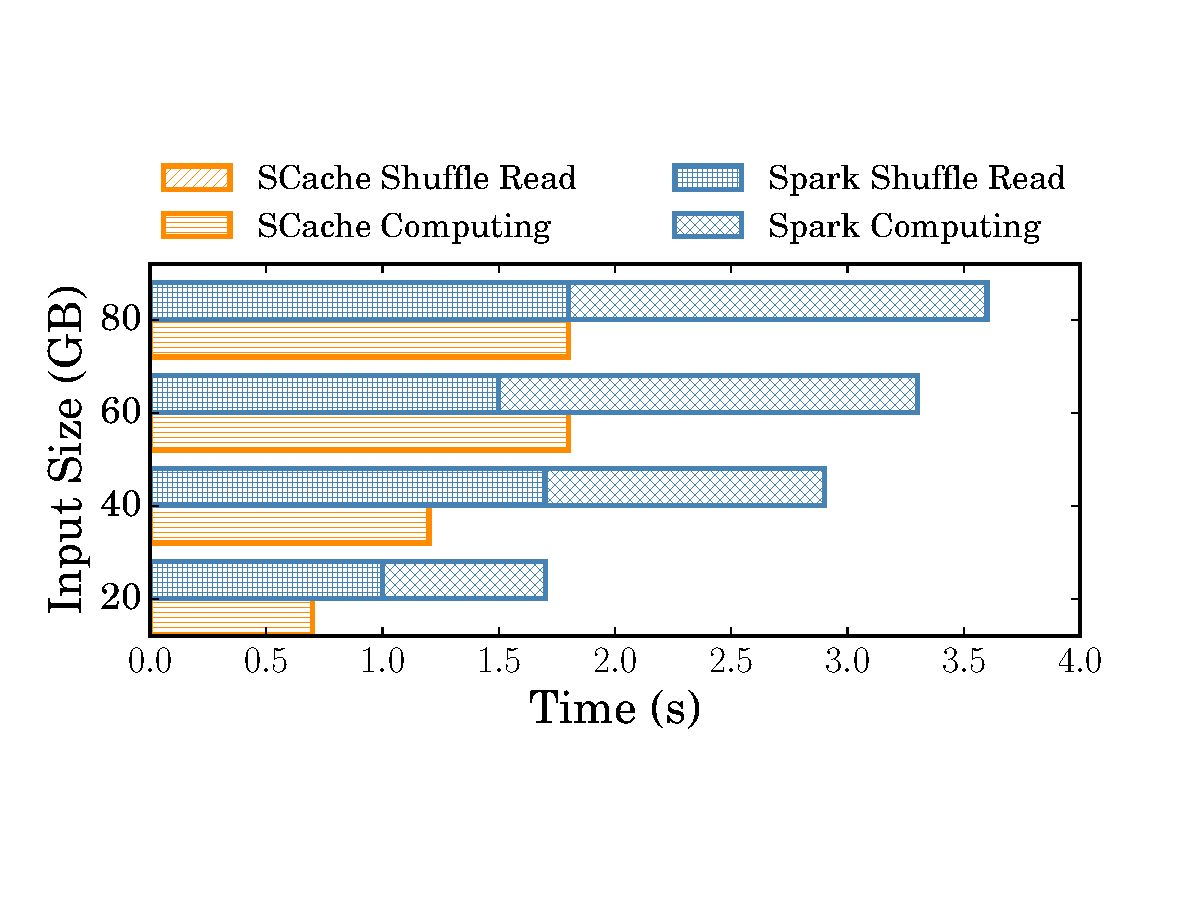
\includegraphics[width=0.6\linewidth]{fig/groupbyreducetask}
% 		\caption{Median Task Details in Reduce Stages}
% 		\label{fig:reducetask}
% 	\end{subfigure}
% 	\caption{Median Task Completion Time of Single Shuffle Test}
% 	\label{fig:singleshuffletask}
% \end{figure}
The performance evaluation in Figure \ref{fig:singleshuffletask} shows the consistent results with our analysis on hardware utilization. For each stage, we run 5 rounds of tasks with different input size. By running spark with SCache, the completion time of map stage can be reduced $10\%$ on average. For reduce stage, instead, SCache achieves a ~$75\%$ performance gain in the completion time of the reduce stage.

A detail analysis into the nutshell of varied overall performance gain on different stages is presented with Figure \ref{fig:singleshuffletask}. For each stage, we pick the median task. About 40\% of shuffle write time can be eliminated by SCache (Figure \ref{fig:maptask}) in a map task. Because the serialization of data is CPU intensive \cite{makingsense} and it is inevitable while moving data out of JVM, SCache can not eliminate the whole phase of shuffle write. It results in a less performance gain in the map stage.
On the other hand, the network transfer introduces a significantly latency in shuffle read of reduce task (Figure \ref{fig:reducetask}). By doing shuffle data pre-fetching for the reduce tasks, the shuffle read time decreases ~$100\%$. That is, the explicit network transfer is perfectly overlapped by SCache shuffle pre-fetching. In overall, SCache can help Spark decrease by ~$89\%$ time in the whole shuffle process. In addition, heuristic reduce tasks scheduling achieves better load balance in cluster than the Spark default FIFO scheduling which may randomly assign two heavy tasks on a single node. So that we can have a significant performance gain in the completion time of the reduce stage.

\subsection{Terasort}
We also evaluate Terasort \cite{spark-tera} --- a recognized shuffle intensive benchmark for distributed system analysis.
Terasort consists of two consecutive shuffles. The first shuffle reads the input data and uses a customized hash partition function for re-partitioning. The second shuffle partitions the data through a range partitioner. As the range bounds set by range partitioner almost match the same pattern of the first shuffle, almost $93\%$ of input data is from one particular map task for each reduce task. So we take the second shuffle as an extreme case to evaluate the scheduling locality for SCache.

As shown in Figure \ref{fig:terasort}, we present the first shuffle as the evaluation of shuffle optimization. At the same time, we use the second shuffle to evaluate in the dimension of scheduling locality (Figure \ref{fig:terashuffle}). For the first shuffle, Spark with SCache runs 2 $\times$ faster during the reduce stage with the input data in a range from 10GB to 200GB. At the same time, Figure \ref{fig:terashuffle} reveals that SCache pre-scheduling produces exactly same network traffic of the second shuffle as Spark, which implies that SCache pre-scheduling can obtain the best locality while balancing the load. In contrast, Spark delays scheduling reduce tasks with the shuffle map output to achieve this optimum.

\begin{figure*}
	\centering
	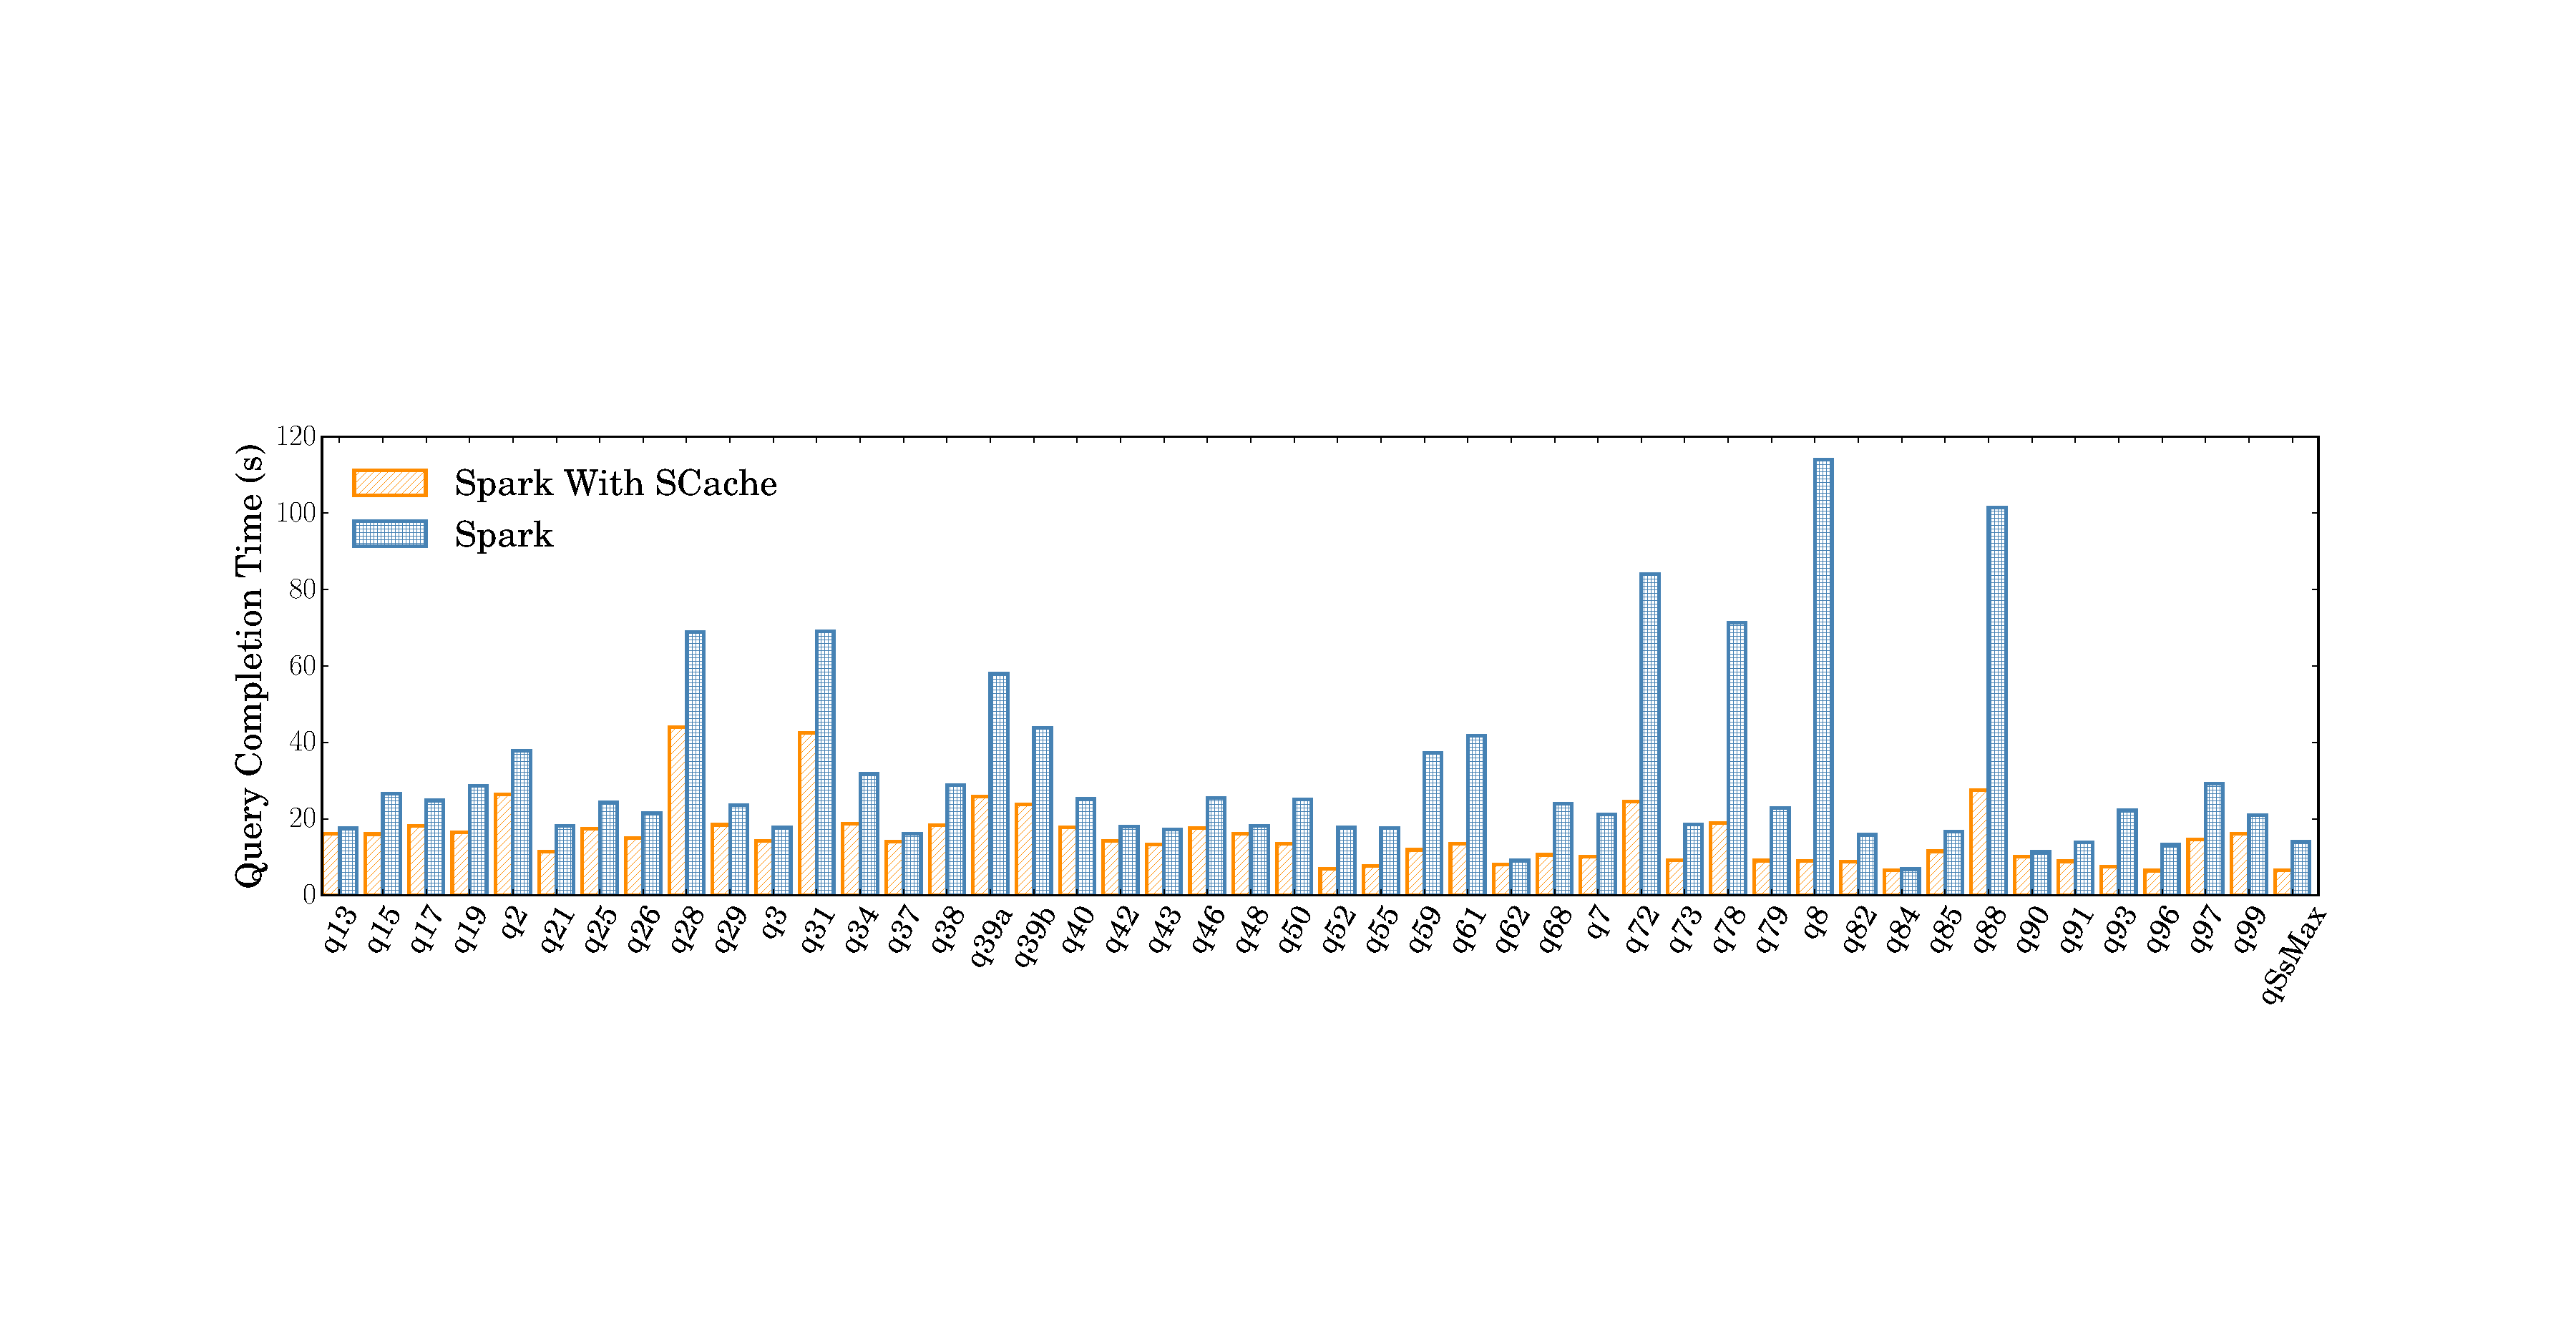
\includegraphics[width=0.85\textwidth]{fig/tpcds}
	\caption{TPC-DS Benchmark Evaluation}
	\label{fig:tpcds}
	\vspace{-1em}
\end{figure*}
\begin{figure}
	\centering
	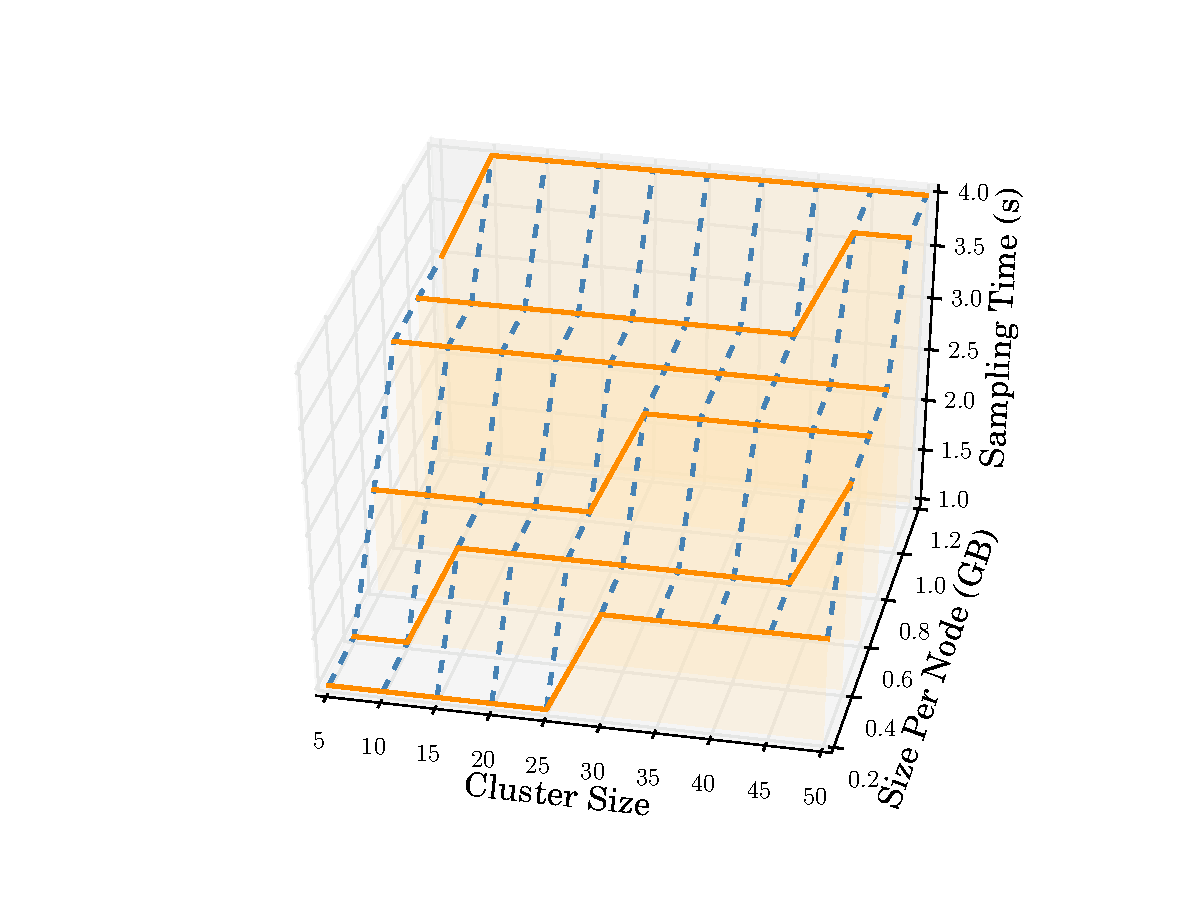
\includegraphics[width=0.6\linewidth]{fig/sampling}
	\caption{Sampling Overhead}
	\label{fig:sampling}
	\vspace{-1em}
\end{figure}

{\color{blue}
\subsection{Hadoop Mapreduce with SCache}

To prove SCache compatibility as a cross-framework plug-in, we also implemented Scache on Hadoop MapReduce as the external shuffle service and co-scheduler. Although \textit{pre-scheduling reduce tasks} is not critical for the simple DAG computing in Hadoop MapReduce, some shuffle-heavy jobs on Hadoop Madpreduce can still be optimized by SCache shuffle data management.

Figure \ref{fig:hadoop_terasort} shows the hardware resource utilization of Hadoop Mapreduce running Terasort. Both figures have the same proportion of time. Hadoop MapReduce with SCache brings 15\% of total time optimization with 384GB input data size. 
As shown in the Figure \ref{fig:hadoop_terasort_origin}, Hadoop Mapreduce without SCache writes intermediate data locally in the Map phase. The shuffle phase and reduce phase start simultaneously. Because the large amount of shuffle data reaches the network bottleneck, The beginning part of reduce needs to wait needs to wait for network transfer. This causes the CPU resources to be idle. 
As shown in the Figure \ref{fig:hadoop_terasort_scache}, Hadoop Madpreduce with SCache start pre-fetching in the Map phase. This avoids the Reduce phase waiting for the shuffle data. Furthermore, pre-fetching utilize the idle IO throughput in the Map phase. As shown in Figure \ref{fig:hadoop_terasort_time}, after better fine-grained utilization of hardware resources, Hadoop Mapreduce with Scache optimize Terasort overall completion time by up to 15\% and an average of 13\% with input data sizes from 128GB to 512GB.
}

\begin{figure}
	\centering
	\begin{minipage}[hb]{\linewidth}
		\begin{subfigure}{\linewidth}
			\begin{minipage}{\linewidth}
				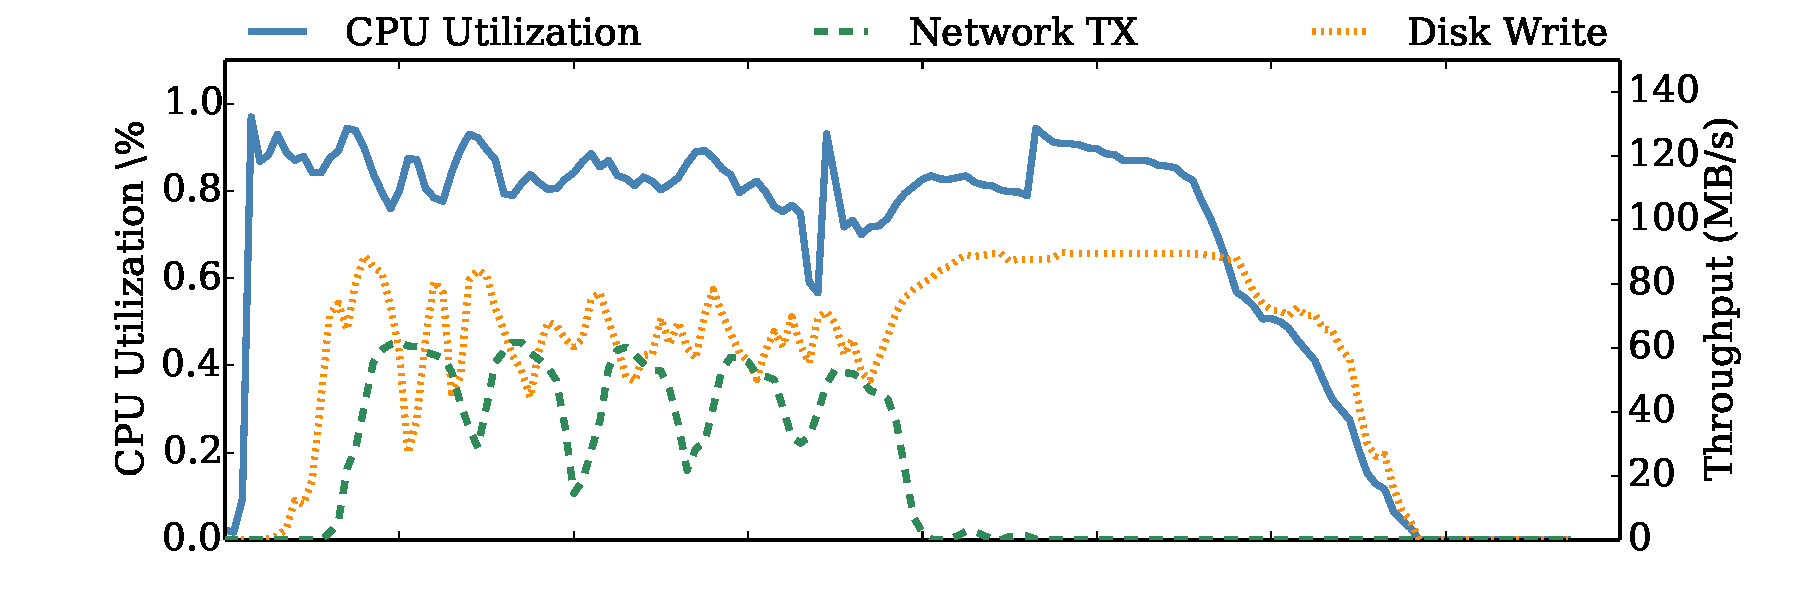
\includegraphics[width=\linewidth]{fig/hadoop_terasort_scache}
				\caption{\color{blue}Hadoop Mapreduce With SCache}
				\label{fig:hadoop_terasort_scache}
			\end{minipage}
			\begin{minipage}{\linewidth}
				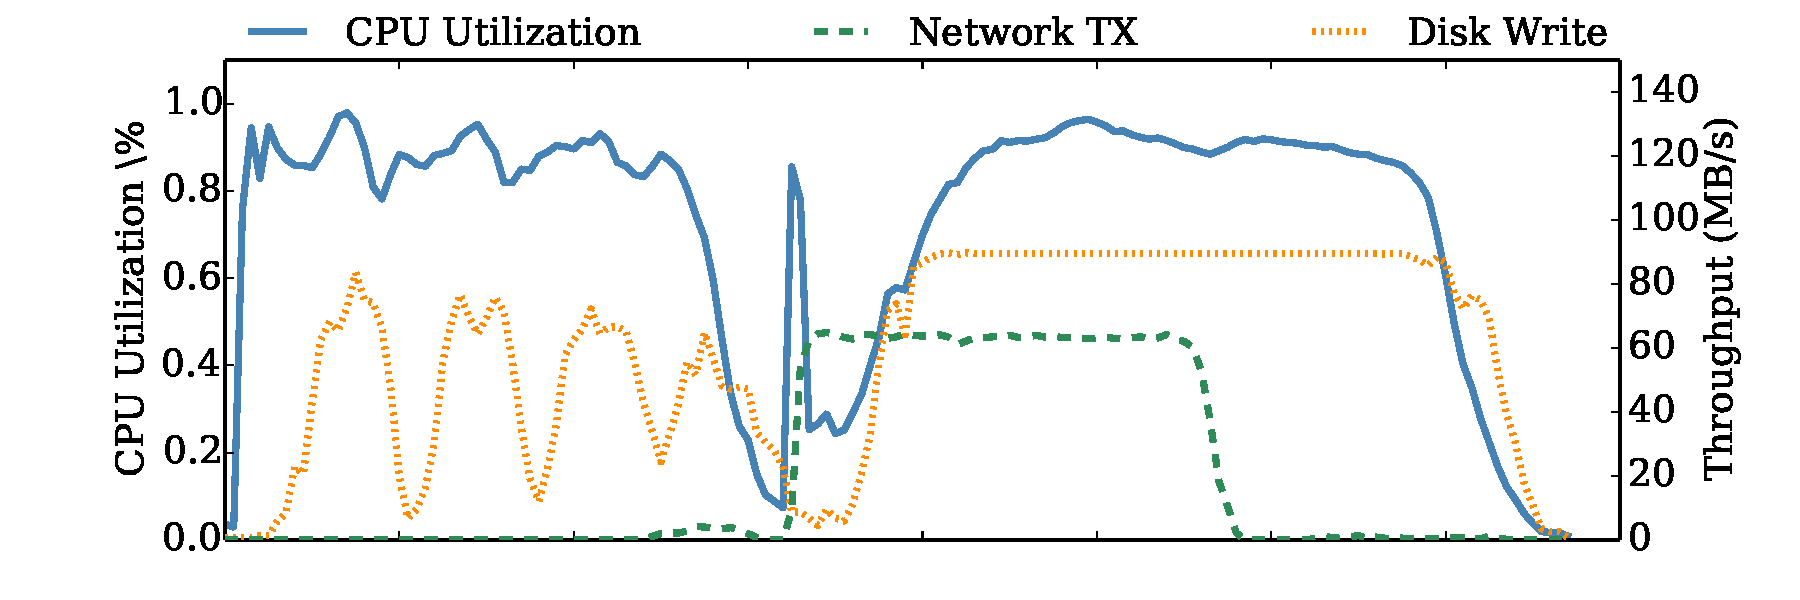
\includegraphics[width=\linewidth]{fig/hadoop_terasort_origin}
				\caption{\color{blue}Hadoop Mapreduce Without SCache}
				\label{fig:hadoop_terasort_origin}
			\end{minipage}
		\end{subfigure}
		\caption{\color{blue}CPU utilization and I/O throughput of a node during a Hadoop Mapreduce Terasort job}
		\label{fig:hadoop_terasort}
	\end{minipage}
\end{figure}

\begin{figure}
	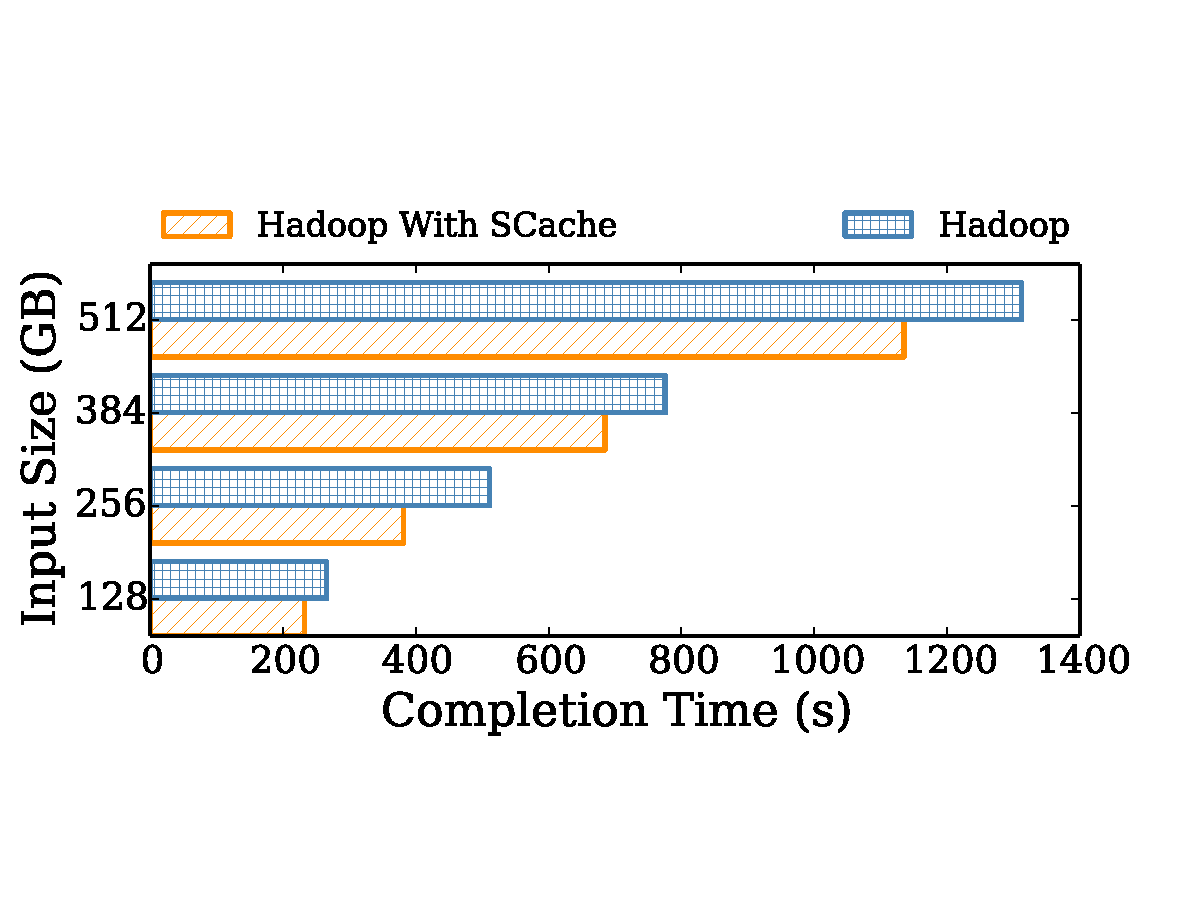
\includegraphics[width=\linewidth]{fig/hadoop_terasort_time}
	\caption{\color{blue}Hadoop Mapreduce Terasort completion time}
	\label{fig:hadoop_terasort_time}
\end{figure}

\subsection{Production Workload}
We also evaluate some shuffle heavy queries from TPC-DS \cite{tpcds}. TPC-DS benchmark is designed for modeling multiple users submitting varied queries (e.g. ad-hoc, interactive OLAP, data mining, etc.). TPC-DS contains 99 queries and is considered as the standardized industry benchmark for testing big data systems. We evaluate the performance of Spark with SCache by picking some of the TPC-DS queries with shuffle intensive attribute. 
As shown in Figure \ref{fig:tpcds}, the horizontal axis is query number, and the vertical axis is query completion time. Spark with SCache outperforms the original Spark in almost all the queries. Furthermore, in many queries, Spark with SCache outperforms original Spark by an order of magnitude. The overall reduction portion of query time that SCache achieved is 40\% on average. Since this evaluation presents the overall job completion time of queries, we believe that our shuffle optimization is promising.
% \begin{figure}
% 	\begin{subfigure}{\linewidth}
% 		\centering
% 		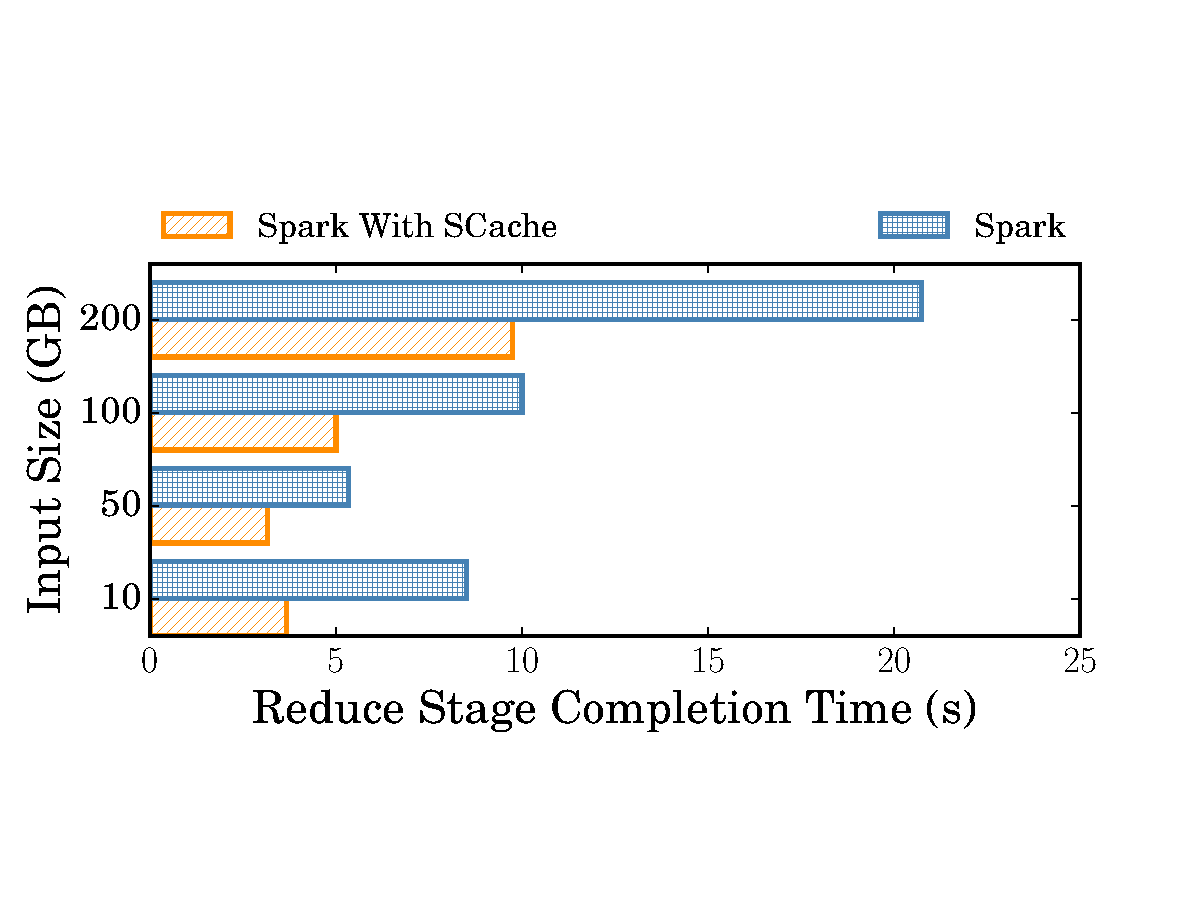
\includegraphics[width=0.6\linewidth]{fig/tera}
% 		\caption{Reduce Stage Completion Time Comparison of First Shuffle}
% 		\label{fig:terasort}
% 	\end{subfigure}
% 	\vspace{0.08cm}
% 	\begin{subfigure}{\linewidth}
% 		\centering
% 		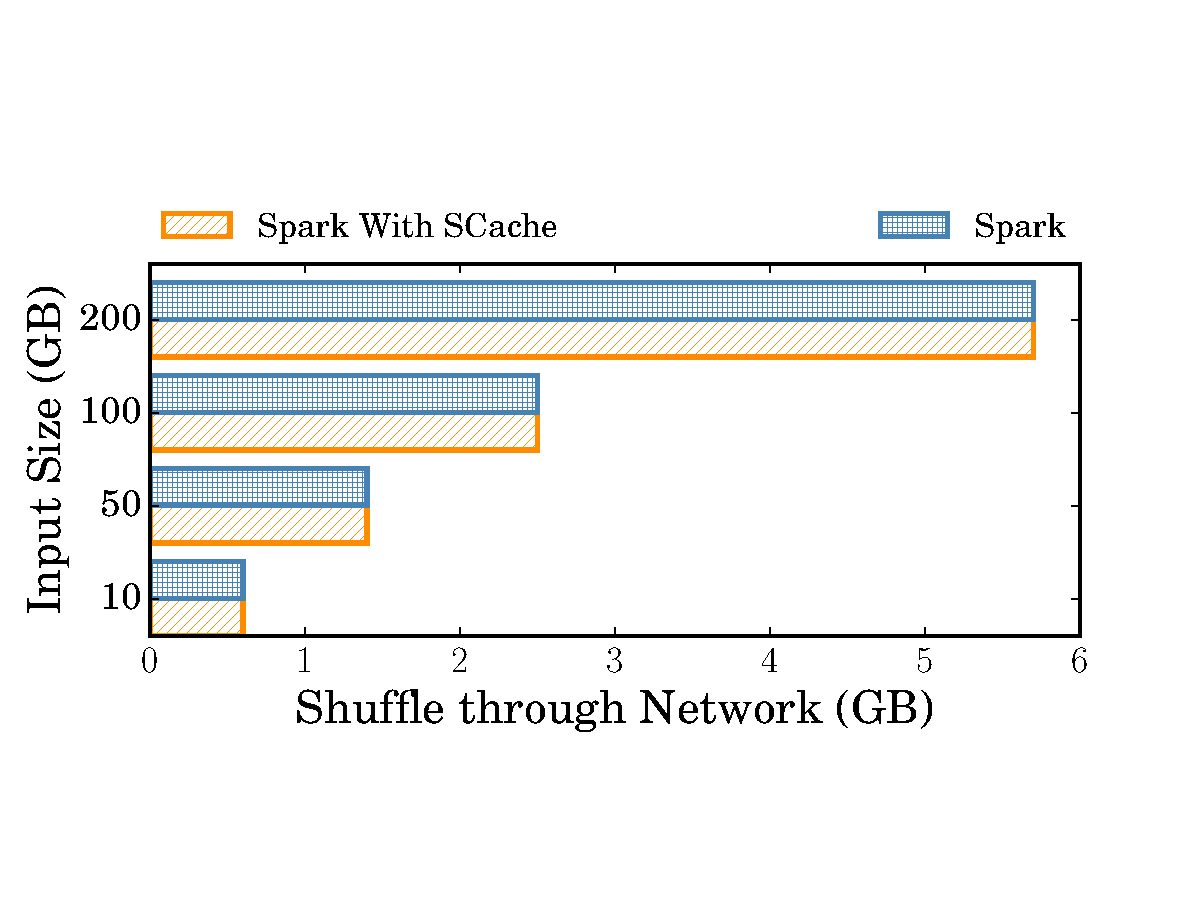
\includegraphics[width=0.6\linewidth]{fig/tera_shuffle}
% 		\caption{Shuffle Data through Network Comparison of Second Shuffle}
% 		\label{fig:terashuffle}
% 	\end{subfigure}
% 	\caption{Terasort Evaluation}
% \end{figure}
\subsection{Overhead of Sampling}
In this part, we evaluate the overhead of sampling with different input data sizes on one node and cluster scales. In Figure \ref{fig:sampling}, the overhead of sampling only grows with the increase of input size on each node. But it remains relatively stable when the cluster size scales up. It makes SCache a scalable system in cluster.
